% TransChromBP Paper Draft v1
% Compile: xelatex transchrombp_paper_draft_v1.tex (twice for references)

\documentclass[11pt,a4paper]{article}

\usepackage[a4paper,margin=1in]{geometry}
\usepackage[colorlinks=true,linkcolor=blue,urlcolor=blue,citecolor=blue]{hyperref}
\usepackage{booktabs}
\usepackage{tabularx}
\usepackage{array}
\usepackage{enumitem}
\usepackage{float}
\usepackage{xcolor}
\usepackage{graphicx}
\usepackage{tikz}
\usepackage{caption}
\usepackage{amsmath}
\usepackage{amssymb}
\usepackage{multirow}
\usepackage{longtable}
\usepackage{authblk}
\usetikzlibrary{arrows.meta,positioning}

\definecolor{goodgreen}{rgb}{0.0,0.5,0.0}
\definecolor{todocolor}{rgb}{0.8,0.0,0.0}
\newcommand{\todo}[1]{\textcolor{todocolor}{[\textbf{TODO}: #1]}}
\newcommand{\pending}[1]{\textcolor{todocolor}{#1}}

%% =====================================================================
\title{TransChromBP: Bias-Safe Transformer Integration \\
for Base-Resolution \\
Chromatin Accessibility Modeling}

\author[1]{Zhengwei Zhou}
\affil[1]{\todo{Affiliation}}
\date{Draft v1 --- March 24, 2026}

%% =====================================================================
\begin{document}
\maketitle

%% =====================================================================
\begin{abstract}
%% =====================================================================

Base-resolution modeling of chromatin accessibility (ATAC-seq) requires
predicting both nucleotide-level profile shapes and total read counts
from DNA sequence alone. ChromBPNet addresses this through bias
factorization, explicitly separating experimental enzymatic bias from
regulatory signal. Meanwhile, Transformer architectures offer a natural
way to capture longer-range genomic dependencies, but their interaction
with bias-factorized profile prediction remains under-characterized.

Here we present TransChromBP, a model that combines convolutional local
encoding, a Transformer backbone, and explicit bias factorization for
ATAC-seq profile/count prediction. In addition to reporting the final
fused output (\emph{full}), we explicitly report the signal-branch-only
output (\emph{debiased}) and use the full/debiased gap as a diagnostic
for bias reliance. A controlled clean-matrix revalidation shows that
when explicit debiased profile supervision is present, both Transformer
and conv-only scaffolds maintain small diagnostic gaps; in contrast,
weakening this supervision increases bias reliance. Importantly, the
largest gap in the current matrix appears in the unsafe conv-only
condition (\(0.02682\)), while the matched unsafe Transformer condition
shows only a mild and stable gap across two seeds (\(0.00972\) and
\(0.00997\)). This evidence does not support a Transformer-specific
shortcut narrative.

On the ENCODE K562 tutorial benchmark, the TransChromBP backbone
achieves \(0.3142 \pm 0.0001\) peak profile JSD and
\(0.8368 \pm 0.0053\) peak count correlation across three seeds. The
final center-pool default model further reaches
\(0.3146 \pm 0.0001\) peak profile JSD and
\(0.8496 \pm 0.0010\) peak count correlation across two held-out seeds,
while retaining a low clean-test gap of \(0.00268\). In the matched
tutorial \texttt{L3} shared-region system compare, TransChromBP also improves
over official ChromBPNet on both peak mean/median JSD
(\(0.31319/0.31547\) vs.\ \(0.33853/0.33989\)) and peak count
correlation (\(0.84016\) vs.\ \(0.69958\)). We further
evaluate integration of a genomic foundation model (Genos-1.2B) and
observe no positive gain, indicating a strong granularity mismatch
between frozen sequence-level summaries and base-resolution prediction.

\end{abstract}

%% =====================================================================
\section{Introduction}
\label{sec:intro}
%% =====================================================================

Chromatin accessibility profiling through assays such as ATAC-seq and
DNase-seq provides a genome-wide readout of open chromatin regions,
which serve as proxies for active regulatory elements including
promoters, enhancers, and transcription factor (TF) binding sites
\cite{buenrostro2013transposition}. Modeling these accessibility signals
at base resolution --- predicting the precise shape of the insertion
profile across each genomic window --- is essential for understanding
fine-grained regulatory mechanisms.

BPNet~\cite{avsec2021base} pioneered base-resolution profile prediction
using dilated convolutional architectures with multinomial profile loss
and total count regression. ChromBPNet~\cite{pampari2023chrombpnet}
extended this framework by introducing \emph{bias factorization}: an
explicit decomposition of the predicted signal into a regulatory
component and an enzymatic bias component. By first pretraining a bias
model on non-peak regions (where signal is dominated by Tn5 insertion
bias), ChromBPNet ensures that the main model learns to predict the
debiased regulatory signal, rather than conflating it with experimental
artifacts. This factorization has proven critical for reliable TF motif
discovery and footprinting analyses.

In parallel, Transformer-based architectures have achieved remarkable
success in genomic sequence modeling. Models such as Enformer
\cite{avsec2021effective}, Nucleotide Transformer
\cite{dallachiesa2023nucleotide}, and the recent Genos
\cite{genos2025} have demonstrated that self-attention mechanisms
can capture long-range regulatory dependencies spanning tens of
kilobases. These advances have naturally raised the question: can
Transformer-based long-range modeling further improve base-resolution
ATAC-seq prediction?

However, combining Transformers with bias factorization is not
straightforward. In early exploratory runs we observed that some
configurations achieved reasonable full profile metrics while their
debiased metrics were markedly worse, suggesting potential reliance on
the bias branch. Rather than treating that exploratory phenomenon as a
mechanistic conclusion a priori, we center this paper on a more careful
question: how should Transformer-enhanced, bias-factorized models be
evaluated so that genuine representational improvement is not confused
with bias reliance?

We present TransChromBP, a model and evaluation framework organized
around that question, with four main contributions:

\begin{enumerate}[leftmargin=2em]
  \item \textbf{Bias-safe Transformer integration.} We combine a
  convolutional local tower, a Transformer sequence encoder, and
  ChromBPNet-style bias factorization in a unified base-resolution ATAC
  model, and show that the Transformer backbone provides a real gain
  over a matched no-Transformer variant.

  \item \textbf{A dual-metric diagnostic framework.} We report both full
  and debiased metrics and use the full/debiased gap as a direct
  diagnostic for bias reliance, rather than relying only on the fused
  output.

  \item \textbf{Controlled clean-matrix revalidation.} We show that
  explicit debiased profile supervision is the more important stabilizer
  in the current framework, while stop-gradient is better understood as
  an auxiliary bias-isolation design. The resulting evidence does not
  support a Transformer-specific shortcut claim.

  \item \textbf{Systematic design study and negative-result analysis.}
  We study backbone ablation, readout-head design, and Genos-1.2B
  integration, reporting both a stable default readout (center pool) and
  a well-characterized negative result for frozen foundation-model
  summary injection.
\end{enumerate}

%% =====================================================================
\section{Results}
\label{sec:results}
%% =====================================================================

All experiments use the ENCODE K562 ATAC-seq tutorial
dataset~\cite{pampari2023chrombpnet}, with held-out test evaluation on
chromosome~1 using the full set of regions (\texttt{nonpeak\_ratio=1.0}).
Unless otherwise noted, we report the mean and standard deviation across
three random seeds (42, 1234, 2024). Primary metrics are peak profile
Jensen-Shannon divergence (JSD, lower is better) and peak count Pearson
correlation ($r$, higher is better).

%% -------------------------------------------------------------------
\subsection{TransChromBP improves over ChromBPNet}
\label{sec:main-result}
%% -------------------------------------------------------------------

Table~\ref{tab:main} uses a dual-track external comparison. Panel A
retains the historical ChromBPNet tutorial baseline, preserving
continuity with the public reference numbers. Panel B reports the newly
closed \texttt{L3} shared-region system compare, where both arms use matched
peaks, non-peaks, and bigWig inputs. These two panels answer different
questions and therefore should not be collapsed into a single ranking.

\begin{table}[H]
\centering
\small
\caption{\textbf{Dual-track external comparison.} Panel A retains the
historical tutorial reference; Panel B gives the matched \texttt{L3}
shared-region system compare.}
\label{tab:main}
\textbf{Panel A. Historical tutorial reference}\\[2mm]
\resizebox{\textwidth}{!}{%
\begin{tabular}{lcccc}
\toprule
Model & Peak profile JSD $\downarrow$ & Aggregation & Peak count $r$ $\uparrow$ & Note \\
\midrule
ChromBPNet (tutorial) & $0.3360$ & median & $0.7274$ & historical external reference \\
TransChromBP corrected B (2 seeds) & $\mathbf{0.3146 \pm 0.0001}$ & mean & $\mathbf{0.8496 \pm 0.0010}$ & default readout \\
\bottomrule
\end{tabular}
}

\vspace{2mm}
\textbf{Panel B. \texttt{L3} shared-region system compare}\\[2mm]
\resizebox{\textwidth}{!}{%
\begin{tabular}{lcccc}
\toprule
Model & Peak mean JSD $\downarrow$ & Peak median JSD $\downarrow$ & Peak count $r$ $\uparrow$ & Note \\
\midrule
Official ChromBPNet controlled L3 & $0.33853$ & $0.33989$ & $0.69958$ & matched peaks/non-peaks/bigWig \\
TransChromBP corrected-B controlled L3 & $\mathbf{0.31319}$ & $\mathbf{0.31547}$ & $\mathbf{0.84016}$ & same shared-region setup \\
\bottomrule
\end{tabular}
}
\end{table}

\noindent Panel A shows that even relative to the historical tutorial
baseline, the paper-facing corrected-B default retains a strong count
advantage ($0.8496$ vs.\ $0.7274$), while the profile column should be
read as a competitive trend because the public baseline reports median
JSD and our default model reports mean JSD. Panel B provides the
stronger controlled evidence: under fully matched shared-region inputs,
TransChromBP improves over official ChromBPNet on peak mean JSD
($-0.02534$), peak median JSD ($-0.02442$), and peak count correlation
($+0.14058$). The paper's external-comparison claim should therefore be
anchored in the combination of historical tutorial continuity and the
matched shared-region comparison, not in the old single-track baseline
alone.

\subsection{Supplementary classification comparison on shared-region L3}
\label{sec:l3-classification}

As a supplementary-style auxiliary comparison, we also report
peak-vs.-nonpeak classification metrics on the \texttt{L3} shared-region test
set (Table~\ref{tab:l3-classification}). These metrics are not promoted
to the main table, but they agree with the profile/count direction:
TransChromBP outperforms official ChromBPNet on AUROC, AUPRC, and best
F1.

\begin{table}[H]
\centering
\small
\caption{\textbf{Supplementary-style classification comparison on \texttt{L3}
shared-region.}}
\label{tab:l3-classification}
\begin{tabular}{lccc}
\toprule
Model & AUROC $\uparrow$ & AUPRC $\uparrow$ & Best F1 $\uparrow$ \\
\midrule
Official ChromBPNet controlled L3 & $0.82295$ & $0.83148$ & $0.75248$ \\
TransChromBP corrected-B controlled L3 & $\mathbf{0.87861}$ & $\mathbf{0.87530}$ & $\mathbf{0.80991}$ \\
\bottomrule
\end{tabular}
\end{table}

%% -------------------------------------------------------------------
\subsection{Transformer provides independent benefit}
\label{sec:tf-ablation}
%% -------------------------------------------------------------------

To isolate the Transformer's contribution from other design choices, we
compare the full TransChromBP architecture (V2-full) with a matched
variant that removes the Transformer blocks while retaining all other
components including the convolutional backbone, bias factorization, and
the stop-gradient fix (V2-noTF). Both variants are trained for 30 epochs
with identical hyperparameters and three random seeds each.

\begin{table}[H]
\centering
\small
\caption{\textbf{Transformer ablation.} V2-full vs.\ V2-noTF, each with
three random seeds. The full/debiased gap column quantifies the degree
of bias leakage (smaller is better).}
\label{tab:tf-ablation}
\begin{tabular}{lcccc}
\toprule
Variant & Peak JSD $\downarrow$ & Peak count $r$ $\uparrow$
  & Full/debiased gap & Seeds \\
\midrule
V2-full (with TF)
  & $\mathbf{0.31419 \pm 0.00012}$ & $\mathbf{0.83676 \pm 0.00531}$
  & $0.00006$ & 3 \\
V2-noTF
  & $0.32393 \pm 0.00021$ & $0.82503 \pm 0.00489$
  & $0.00010$ & 3 \\
\midrule
$\Delta$ & $-0.00974$ ($-3.0\%$) & $+0.01173$ ($+1.4\%$) & & \\
\bottomrule
\end{tabular}
\end{table}

\noindent V2-full achieves a consistent improvement across all three
seeds: peak JSD decreases by 0.010 (3.0\% relative), and count
correlation increases by 0.012 (1.4\% relative). Critically, the
full/debiased gap remains extremely small (0.00006), confirming that the
Transformer's benefit arises from genuine representational capacity
rather than re-introducing bias leakage. All six comparisons (3 seeds
$\times$ 2 metrics) favor V2-full, yielding a sign-test $p$-value of
$1/64 \approx 0.016$.

%% -------------------------------------------------------------------
\subsection{Bias-reliance diagnostics under clean-matrix revalidation}
\label{sec:shortcut}
%% -------------------------------------------------------------------

In a bias-factorized architecture, reporting only the final fused output
(\emph{full}) is insufficient for deciding whether the signal branch has
actually learned a debiased regulatory representation. We therefore
jointly report:

\begin{itemize}[leftmargin=2em]
  \item \textbf{Full metrics}: computed from the final fused output;
  \item \textbf{Debiased metrics}: computed from the signal branch alone;
  \item \textbf{Full/debiased gap}: a direct diagnostic for extra
  reliance on the bias branch.
\end{itemize}

\noindent Early exploratory runs suggested that some configurations
might have substantial gaps, but those runs also changed multiple design
and training factors simultaneously. The paper-facing conclusion should
therefore be based on the current clean matrix.

\begin{table}[H]
\centering
\small
\caption{\textbf{Clean-matrix revalidation for bias reliance.} Under
explicit debiased supervision, both TF and conv-only scaffolds remain
clean. Under the unsafe setting (\texttt{sg=true, deb0}), the
Transformer cell shows only a mild and stable gap across two seeds,
whereas the matched conv-only cell shows the largest gap in the matrix.}
\label{tab:shortcut}
\resizebox{\textwidth}{!}{%
\begin{tabular}{lccccc}
\toprule
Run & Condition & Peak JSD (full) & Peak JSD (debiased) & Gap & Peak count $r$ (full/deb) \\
\midrule
A & \texttt{TF + sg=false + deb2} & $0.31410$ & $0.31416$ & $0.00147$ & $0.8506 / 0.8488$ \\
C (2 seeds) & \texttt{TF + sg=true + deb0} & $0.31730 \pm 0.00014$ & $0.31787 \pm 0.00011$ & $0.00984 \pm 0.00018$ & $0.8367 \pm 0.0039 / 0.8348 \pm 0.0031$ \\
noTF-safe & \texttt{noTF + sg=false + deb2} & $0.43531$ & $0.43557$ & $0.00487$ & $0.7959 / 0.7966$ \\
noTF-unsafe & \texttt{noTF + sg=true + deb0} & $0.43659$ & $0.43835$ & $0.02682$ & $0.7919 / 0.7956$ \\
corrected B & \texttt{TF + center + sg=true + deb2} & $0.42544$ & $0.42556$ & $0.00268$ & $0.8439 / 0.8420$ \\
\bottomrule
\end{tabular}
}
\end{table}

\noindent Three conclusions follow.

First, the current evidence does \emph{not} support a
Transformer-specific strong-shortcut story. The unsafe Transformer cell
(C) shows only a mild gap, albeit one that is stable across two seeds
(\(0.00972\) and \(0.00997\)). The largest gap in the matrix instead
appears in the matched unsafe conv-only condition (\(0.02682\)).

Second, the clean matrix supports a supervision-driven interpretation.
Condition A remains extremely clean even without stop-gradient, whereas
C becomes noticeably gap-prone despite retaining stop-gradient. This
indicates that explicit debiased profile supervision is the more
important stabilizer in the current framework, while stop-gradient is
better interpreted as an auxiliary bias-isolation design.

Third, the paper-facing final model (\emph{corrected B}) also remains
clean, with a gap of only \(0.00268\). This matters for the paper story:
the final model is not improving by leaning harder on the bias branch;
it improves count prediction while remaining diagnostically safe.

%% -------------------------------------------------------------------
\subsection{Component ablation}
\label{sec:ablation}
%% -------------------------------------------------------------------

Table~\ref{tab:ablation} presents a systematic ablation removing each
major component from the full TransChromBP model.

\begin{table}[H]
\centering
\small
\caption{\textbf{Component ablation.} Each row removes one component
from the current default model. $^\dag$3-seed mean; $^\ddag$2-seed mean.}
\label{tab:ablation}
\begin{tabular}{llccc}
\toprule
Variant & What is removed & Peak JSD $\downarrow$ & Peak count $r$ $\uparrow$
  & Seeds \\
\midrule
TransChromBP (full)$^\ddag$
  & --- & $\mathbf{0.3146 \pm 0.0001}$ & $\mathbf{0.8496 \pm 0.0010}$ & 2 \\
\quad w/o center pool$^\dag$
  & Center-aligned count pool & $0.3142 \pm 0.0001$ & $0.8368 \pm 0.0053$ & 3 \\
\quad w/o Transformer$^\dag$
  & Transformer blocks & $0.3239 \pm 0.0002$ & $0.8250 \pm 0.0049$ & 3 \\
\midrule
ChromBPNet (reference)
  & --- & $0.3360$ & $0.7274$ & 1 \\
\bottomrule
\end{tabular}
\end{table}

Key observations from the ablation:

\begin{itemize}[leftmargin=2em]
  \item \textbf{Transformer is the largest single contributor.} Removing
  the Transformer increases peak JSD by 0.010 (3\%) and decreases count
  $r$ by 0.012, the largest effect among all ablations.

  \item \textbf{Center pool provides a consistent count improvement.}
  Relative to the backbone scaffold without center-aligned pooling, the
  corrected-B default model improves count $r$ by roughly 0.013 while
  preserving the same profile JSD regime.

  \item \textbf{Bias-safe supervision should be discussed from the clean
  matrix, not this table alone.} The supervision question is better
  answered by the explicit full/debiased diagnostic matrix in
  Table~\ref{tab:shortcut}, where unsafe TF and unsafe noTF settings are
  compared directly.
\end{itemize}

%% -------------------------------------------------------------------
\subsection{Readout head design}
\label{sec:readout}
%% -------------------------------------------------------------------

We evaluated four readout head variants to understand how the mapping
from Transformer representations to final predictions affects
performance (Table~\ref{tab:readout}). All variants share the same
Transformer backbone and bias-safe training framework, differing only in
the count pooling strategy and/or profile head architecture.

\begin{table}[H]
\centering
\small
\caption{\textbf{Readout head comparison.} All variants trained for
40 epochs with seed 42. The baseline uses global mean pooling.}
\label{tab:readout}
\begin{tabular}{llccc}
\toprule
Variant & Design & Peak JSD $\downarrow$ & Peak count $r$ $\uparrow$
  & Best epoch \\
\midrule
A: Freeze fix & Frozen bias BN & $0.3148$ & $0.8446$ & 40 \\
B: Center pool & Center-aligned count & $\mathbf{0.3147}$ & $\mathbf{0.8503}$ & 34 \\
F: Attention pool & Attention-weighted count & $0.3148$ & $0.8492$ & 40 \\
G: Profile refine & Learned profile head & $0.4260$ & $0.8460$ & 15 \\
\midrule
Baseline & Global mean pool & $0.3143$ & $0.8354$ & 29 \\
\bottomrule
\end{tabular}
\end{table}

\noindent On seed 42 alone, variants A, B, and F all improve count
correlation substantially over the baseline ($+0.009$ to $+0.015$) while
maintaining nearly identical profile JSD ($0.3147$--$0.3148$). However,
the matched seed-1234 confirmatory runs separate B from F: B remains
stable (\(0.3145 / 0.8488\)), whereas F degrades sharply on profile
JSD (\(0.4269\)) despite retaining reasonable count performance
(\(0.8457\)). This makes center pool the only readout option that
remains stable across the currently available confirmatory seeds.

Variant G (profile refine) represents a cautionary case: adding a learnable
profile head produces reasonable count correlation but dramatically
worsens profile JSD, suggesting that the additional parameters overfit
to training-distribution profile shapes. The early best epoch (15 vs.\
29--40 for other variants) further supports this interpretation.

%% -------------------------------------------------------------------
\subsection{Genomic foundation model integration yields no positive gain}
\label{sec:genos}
%% -------------------------------------------------------------------

Motivated by the success of pretrained genomic foundation models in
sequence-level tasks, we investigated whether Genos-1.2B \cite{genos2025}
embeddings could provide additional benefit to TransChromBP. We evaluated
five integration strategies spanning two paradigms:
\emph{online fusion} (Genos runs during training) and
\emph{cached fusion} (precomputed Genos summaries).

\begin{table}[H]
\centering
\small
\caption{\textbf{Foundation model integration.} All variants compared
against the matched G0 baseline. No variant achieves positive gain on
both metrics simultaneously.}
\label{tab:genos}
\begin{tabular}{llcc}
\toprule
Recipe & Strategy & Peak JSD $\downarrow$ & Peak count $r$ $\uparrow$ \\
\midrule
G0 (baseline) & No Genos & $0.3163$ & $\mathbf{0.8410}$ \\
\midrule
G1 (gate) & Online, per-position gate & $0.3388$ & $0.4689$ \\
G2 (mean) & Online, global mean & $0.3387$ & $0.6360$ \\
P0 (cached baseline) & Cached, matched config & $0.3179$ & $0.8384$ \\
P2 (count-only) & Cached, count head inject & $\mathbf{0.3174}$ & $0.6037$ \\
\bottomrule
\end{tabular}
\end{table}

\noindent None of the five strategies produces a positive result.
Online fusion (G1, G2) causes catastrophic count collapse on held-out
test despite appearing reasonable during validation, exposing a
severe generalization failure. Cached fusion with matched baseline (P0)
is stable but does not improve over G0. Cached count-only injection (P2)
achieves the best profile JSD but causes a severe count collapse
($r = 0.60$), indicating that injecting a coarse global summary directly
into the count head is destructive.

\subsubsection{Why the foundation model does not help}

To understand this negative result, we conducted a diagnostic probe
on the cached Genos summaries:

\begin{itemize}[leftmargin=2em]
  \item \texttt{genos\_only} achieves AUC $= 0.70$ for peak vs.\ non-peak
  classification, confirming that the Genos summary contains accessibility-related
  information.
  \item However, \texttt{concat(encoded, genos)} achieves AUC $= 0.90$,
  which is \emph{lower} than \texttt{encoded\_only} at AUC $= 0.92$.
  \item The Genos summary explains only $R^2 = 0.017$ of the count
  residual (after accounting for the model's own prediction).
\end{itemize}

\noindent These probes reveal that while Genos embeddings contain
genuine accessibility information, this information largely overlaps
with what the task-specific backbone already captures, and na\"ive
concatenation introduces noise rather than complementary signal.

To verify that this negative result reflects a task-level mismatch
rather than an implementation failure, we reproduced the official Genos
OCR (open chromatin region) classification benchmark, achieving
AUC $= 0.7535$ with layer 12 embeddings --- within 0.5\% of the
published value of 0.7569. This confirms that the local Genos
installation and inference pipeline are correct; the failure is specific
to the base-resolution profile/count prediction task.

The fundamental issue is a \emph{granularity mismatch}: the OCR
benchmark is a sequence-level binary classification task naturally suited
to global mean-pooled summaries, whereas ATAC profile prediction requires
base-resolution spatial information about local motif composition and
positional structure --- information that is lost in the global pooling
step.

%% -------------------------------------------------------------------
\subsection{Multi-dataset generalization}
\label{sec:multi-dataset}
%% -------------------------------------------------------------------

To verify that TransChromBP generalizes beyond the tutorial dataset, we
trained models on two independent ENCODE ATAC-seq datasets: GM12878 and
K562 (distinct from the tutorial K562 data, using a different replicate
configuration and preprocessing pipeline).

\begin{table}[H]
\centering
\small
\caption{\textbf{Multi-dataset generalization.} Both datasets show
consistent validation-to-test agreement, confirming no split-specific
overfitting. These are 6002 single-GPU runs, and absolute JSD values
should not be compared across datasets because the peak sets and signal
distributions differ.}
\label{tab:multi-dataset}
\begin{tabular}{lcccc}
\toprule
Dataset & Best epoch & Val peak JSD & Test peak JSD & Test peak count $r$ \\
\midrule
GM12878 & 19 & $0.4302$ & $0.4226$ & $0.8040$ \\
K562 & 35 & $0.6281$ & $0.6124$ & $0.8586$ \\
\bottomrule
\end{tabular}
\end{table}

\noindent In both cases, held-out test performance meets or exceeds
validation performance, indicating that the model does not exhibit
split-specific overfitting. The higher absolute JSD values for these
datasets likely reflect differences in peak characteristics and
signal-to-noise ratios rather than model failure.

%% =====================================================================
\section{Discussion}
\label{sec:discussion}
%% =====================================================================

%% -------------------------------------------------------------------
\subsection{Bias-reliance diagnostics as a design principle}
%% -------------------------------------------------------------------

The main methodological lesson of this work is not that we have proven a
strong, Transformer-specific shortcut mechanism. Rather, it is that
whenever a model combines a high-capacity sequence backbone with an
explicit auxiliary bias/confound branch, \emph{full-only reporting can be
misleading}. The full/debiased gap provides a low-cost, directly
interpretable diagnostic for whether apparent performance gains are
coming from the intended signal pathway.

The clean matrix also sharpens the boundary of what we can claim. The
current evidence supports saying that explicit debiased profile
supervision is important for stable training, and that the final
paper-facing model remains diagnostically clean. It does \emph{not}
support saying that we have proven a universal Transformer-specific
failure mode. In fact, the currently largest gap appears in the unsafe
conv-only condition.

Our finalized single-seed no-bias supplementary run (\texttt{2026-03-31}) also
helps define that boundary. Using the current tutorial-canonical
paper-facing recipe plus an external valid selector, the no-bias model
selected \texttt{epoch 26}; on held-out \texttt{test-full}, it reached peak
mean/median JSD=\texttt{0.31496/0.31715}, peak count $r$=\texttt{0.84978}, and
count-scale peak-vs.-nonpeak \texttt{AUROC/AUPRC/best F1 =
0.88990/0.88418/0.82037}. These numbers are essentially in the same
band as the current corrected-B / center-pool configuration. This does
not support writing that removing the bias branch causes a clear drop,
nor that it yields a clearly stronger model. The more accurate reading
is that, under the current Transformer + center-pool recipe, explicit
bias factorization does not show a clear extra benefit in this
single-seed boundary check; however, that result still does not replace
the clean matrix as the bias-safety diagnostic or the \texttt{L3}
shared-region comparison as the main external evidence.

This is still useful as a broader design principle: future
bias-factorized genomic models should report both fused and debiased
outputs whenever the architecture contains an explicit auxiliary branch
with learnable fusion, regardless of whether the backbone is a
Transformer.

%% -------------------------------------------------------------------
\subsection{Foundation models and task granularity}
%% -------------------------------------------------------------------

Our Genos-1.2B experiments provide a well-controlled negative result for
the genomics community. The key insight is that foundation model
effectiveness depends critically on the \emph{granularity match} between
pretraining and downstream tasks:

\begin{itemize}[leftmargin=2em]
  \item For sequence-level classification (e.g., OCR detection), global
  mean-pooled embeddings work well, as confirmed by our OCR benchmark
  reproduction.
  \item For base-resolution regression (e.g., ATAC profile prediction),
  the same embeddings lose the spatial information that is critical for
  the task.
\end{itemize}

\noindent This does not imply that foundation models are useless for
profile prediction --- but it does imply that the integration strategy
must preserve spatial resolution, potentially through per-position
features, cross-attention, or fine-tuning rather than frozen summary
injection.

Furthermore, the strong task-specific baseline achieved by TransChromBP
leaves little room for incremental improvement from external embeddings.
When the baseline is weak, even noisy external features can help;
when the baseline is strong and task-specialized, the bar for external
contribution is correspondingly high.

%% -------------------------------------------------------------------
\subsection{Limitations and future work}
%% -------------------------------------------------------------------

Several limitations of this work suggest directions for future research:

\begin{itemize}[leftmargin=2em]
  \item \textbf{Single primary benchmark.} Our main ablations use a
  single ENCODE K562 ATAC-seq dataset. While the multi-dataset
  experiments (GM12878, K562) demonstrate generalization, a comprehensive
  evaluation across more cell types and assays (DNase-seq) would
  strengthen the conclusions.

  \item \textbf{No distillation.} The current framework uses direct
  training only. Teacher-student distillation, where a larger or
  longer-context teacher guides a compact student, could potentially
  amplify the Transformer's benefit while maintaining efficiency.

  \item \textbf{Foundation model integration.} We only tested frozen
  global summary injection. More sophisticated strategies (per-position
  features, cross-attention, LoRA fine-tuning) might unlock the spatial
  information in foundation model representations.

  \item \textbf{Input window length.} TransChromBP uses the same 2114\,bp
  window as ChromBPNet. Extending to longer windows could increase the
  Transformer's comparative advantage, though this requires corresponding
  changes to data preprocessing and training infrastructure.

  \item \textbf{Variance in the unsafe conv-only cell.} The
  \texttt{noTF + sg=true + deb0} condition is already informative enough
  to reject a Transformer-specific shortcut story, but its paper-facing
  matrix entry is currently based on a single completed test seed. More
  seeds would tighten the variance estimate for that cell.

  \item \textbf{External baseline aggregation mismatch.} The public
  ChromBPNet tutorial reports peak profile median JSD, whereas our main
  TransChromBP tables report mean JSD. The count comparison is directly
  comparable; the profile comparison should be interpreted more
  conservatively.
\end{itemize}

%% =====================================================================
\section{Methods}
\label{sec:methods}
%% =====================================================================

%% -------------------------------------------------------------------
\subsection{Model architecture}
\label{sec:arch}
%% -------------------------------------------------------------------

TransChromBP (Figure~\ref{fig:arch})
takes a one-hot encoded DNA sequence of length $L = 2114$\,bp as input
and produces two outputs: a base-resolution profile prediction over the
central 1000\,bp window, and a scalar log-count prediction.

\begin{figure}[H]
\centering
\resizebox{\textwidth}{!}{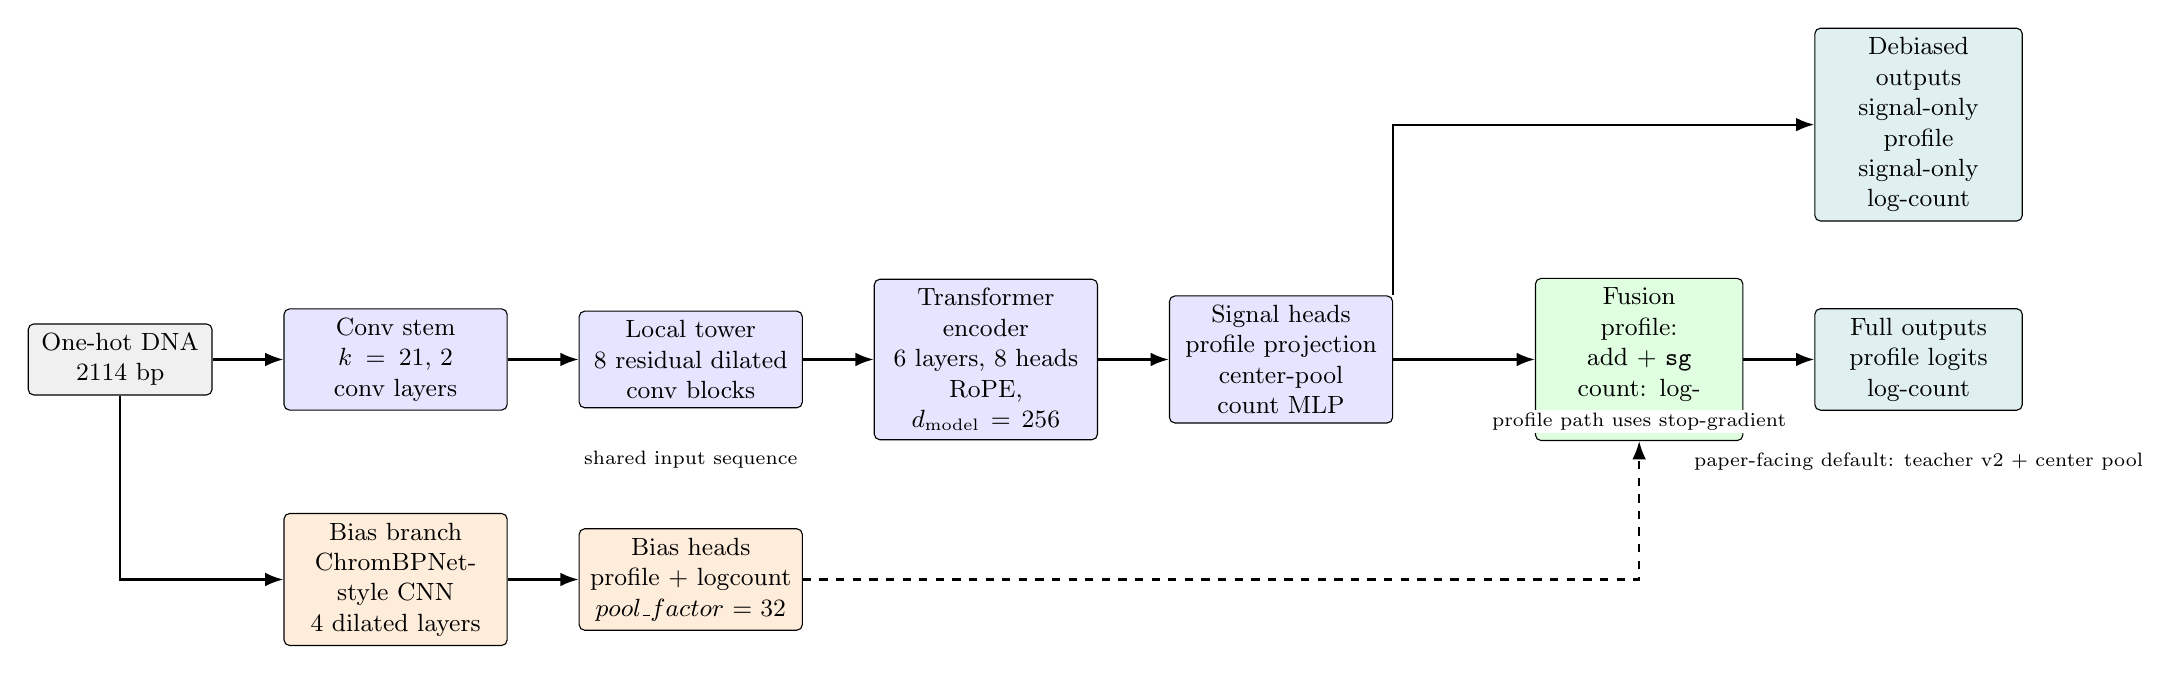
\begin{tikzpicture}[
  font=\small,
  >=Latex,
  node distance=7mm and 9mm,
  data/.style={draw, rounded corners=2pt, align=center, minimum height=9mm, text width=21mm, fill=gray!12},
  sig/.style={draw, rounded corners=2pt, align=center, minimum height=9mm, text width=26mm, fill=blue!10},
  bias/.style={draw, rounded corners=2pt, align=center, minimum height=9mm, text width=26mm, fill=orange!14},
  fuse/.style={draw, rounded corners=2pt, align=center, minimum height=9mm, text width=24mm, fill=green!12},
  outbox/.style={draw, rounded corners=2pt, align=center, minimum height=9mm, text width=24mm, fill=teal!12},
  arrow/.style={-Latex, thick},
  sg/.style={-Latex, thick, dashed},
  note/.style={font=\scriptsize, inner sep=1pt, fill=white}
]

\node[data] (dna) {One-hot DNA\\2114 bp};

\node[sig, right=of dna] (stem) {Conv stem\\$k=21$, 2 conv layers};
\node[sig, right=of stem] (tower) {Local tower\\8 residual dilated\\conv blocks};
\node[sig, right=of tower] (tf) {Transformer encoder\\6 layers, 8 heads\\RoPE, $d_{\text{model}}=256$};
\node[sig, right=of tf] (signal) {Signal heads\\profile projection\\center-pool count MLP};

\node[bias, below=13mm of stem] (biasnet) {Bias branch\\ChromBPNet-style CNN\\4 dilated layers};
\node[bias, right=of biasnet] (biasheads) {Bias heads\\profile + logcount\\$pool\_factor=32$};

\node[fuse, right=18mm of signal] (fusion) {Fusion\\profile: add + \texttt{sg}\\count: log-sum-exp};
\node[outbox, right=of fusion] (full) {Full outputs\\profile logits\\log-count};
\node[outbox, above=11mm of full] (deb) {Debiased outputs\\signal-only profile\\signal-only log-count};

\draw[arrow] (dna) -- (stem);
\draw[arrow] (stem) -- (tower);
\draw[arrow] (tower) -- (tf);
\draw[arrow] (tf) -- (signal);

\draw[arrow] (dna.south) |- (biasnet.west);
\draw[arrow] (biasnet) -- (biasheads);

\draw[arrow] (signal) -- (fusion);
\draw[sg] (biasheads.east) -| (fusion.south);
\node[note, above=1mm of fusion.south] {profile path uses stop-gradient};

\draw[arrow] (fusion) -- (full);
\draw[arrow] (signal.north east) |- (deb.west);

\node[note, below=5mm of tower] {shared input sequence};
\node[note, below=5mm of full] {paper-facing default: teacher v2 + center pool};

\end{tikzpicture}
}
\caption{\textbf{Paper-facing TransChromBP architecture.} The signal
branch combines a convolutional stem, an 8-layer local dilated tower,
and a 6-layer Transformer encoder; the bias branch is a smaller
ChromBPNet-style CNN. Bias profile contributions enter the fused profile
through stop-gradient, whereas counts are combined by log-sum-exp in log
space.}
\label{fig:arch}
\end{figure}

\subsubsection{Convolutional stem and local tower}

The input sequence $\mathbf{x} \in \{0,1\}^{L \times 4}$ is first
processed by a convolutional stem consisting of a 1D convolution
(kernel size 21, $d_{\text{model}}=256$ output channels), GELU
activation, and 0.1 dropout. This is followed by a local tower of
eight residual dilated convolutional blocks with exponentially
increasing dilation rates ($2^0, 2^1, \ldots, 2^7$), capturing local
motif patterns and short-range interactions. After the stem, two
additional convolutional layers with kernel size 7 are retained for
local mixing.

\subsubsection{Transformer encoder}

The local tower output is passed to a Transformer encoder with
rotary position embeddings (RoPE). The encoder consists of 6 layers of
multi-head self-attention with 8 heads, pre-norm (LayerNorm),
GELU-gated feed-forward networks, and residual connections. The
feed-forward dimension is $d_{\text{ff}} = 4d_{\text{model}} = 1024$,
and dropout is fixed at 0.1 throughout the encoder.

\subsubsection{Output heads}

The Transformer output is mapped to predictions through two heads:

\begin{itemize}[leftmargin=2em]
  \item \textbf{Profile head.} A linear projection from $d_{\text{model}}$
  to 1, applied independently at each position, followed by center
  cropping to 1000\,bp. The output represents unnormalized log-probabilities
  (logits) for a multinomial distribution over positions.

  \item \textbf{Count head.} The encoded representation is pooled over
  the center 1000\,bp window (center pool), then passed through a
  two-layer MLP: LayerNorm $\to$ Linear($d_{\text{model}}$,
  $d_{\text{model}}/2$) $\to$ GELU $\to$ Dropout $\to$ Linear $\to$
  scalar log-count.
\end{itemize}

\subsubsection{Bias factorization}

An independent bias branch models the enzymatic bias signal. It
consists of a smaller convolutional network (stem + dilated tower)
with separate profile and count heads. The bias branch is first
pretrained on non-peak regions (where signal is dominated by Tn5
insertion bias), then its core parameters are frozen while learnable
scale parameters $\alpha_p$ and $\alpha_c$ (initialized to 1.0,
constrained positive via softplus) modulate its contribution to the
final prediction:

\begin{align}
  \text{profile}_{\text{full}} &= \text{profile}_{\text{signal}}
    + \alpha_p \cdot \texttt{sg}(\text{profile}_{\text{bias}})
    \label{eq:fusion-profile} \\
  \text{logcount}_{\text{full}} &= \log\bigl(
    \exp(\text{logcount}_{\text{signal}})
    + \alpha_c \cdot \exp(\text{logcount}_{\text{bias}})
  \bigr)
    \label{eq:fusion-count}
\end{align}

\noindent where $\texttt{sg}(\cdot)$ denotes stop-gradient, meaning
that gradients are blocked from flowing back into the frozen bias
branch through the profile fusion path. The count fusion uses
log-sum-exp to combine contributions in log space.

%% -------------------------------------------------------------------
\subsection{Training procedure}
\label{sec:training}
%% -------------------------------------------------------------------

Training proceeds in two stages:

\begin{enumerate}[leftmargin=2em]
  \item \textbf{Bias pretraining.} The bias branch is trained on
  non-peak regions for a fixed number of epochs, learning to predict
  the enzymatic bias signal.

  \item \textbf{Main training.} The full model is trained on both peak
  and non-peak regions, with the bias branch core frozen and only the
  scale parameters, signal branch, and Transformer being updated.
\end{enumerate}

\noindent The main training loss is:
\begin{equation}
  \mathcal{L} = \mathcal{L}_{\text{profile}} + \lambda_c \cdot \mathcal{L}_{\text{count}}
\end{equation}
where $\mathcal{L}_{\text{profile}}$ is the multinomial negative
log-likelihood over the central 1000\,bp profile, and
$\mathcal{L}_{\text{count}}$ is the mean squared error on the
log-count. The count loss weight $\lambda_c$ is calibrated
automatically.

Optimization uses AdamW with learning rate $5\times 10^{-4}$, weight
decay 0.01, and $\beta=(0.9, 0.95)$, together with a cosine schedule, a
warmup ratio of 0.06, and a minimum learning-rate ratio of 0.1. Early
stopping is based on validation peak profile JSD. Tutorial backbone and
clean-matrix runs typically use 30 epochs; readout-head closure uses 40
epochs; the shared-region strict compare uses 50 epochs. Two-GPU runs
use \texttt{batch\_size\_per\_gpu=16} (effective batch size 32), whereas 6000
single-GPU confirmatory runs keep the same effective batch through
\texttt{grad\_accum=2}. Data augmentation includes $\pm 500$\,bp random jitter
and reverse-complement augmentation with probability 0.5.

%% -------------------------------------------------------------------
\subsection{Data and preprocessing}
\label{sec:data}
%% -------------------------------------------------------------------

\subsubsection{Primary benchmark}

We use the ENCODE K562 ATAC-seq dataset from the ChromBPNet tutorial
\cite{pampari2023chrombpnet}, consisting of merged BAM files from
three biological replicates. Peaks are summit-centered, non-peaks are
GC-matched negatives, and the signal is an unstranded insertion bigWig.
Chromosome splits follow the standard ChromBPNet fold configuration:
chromosomes are partitioned into training, validation, and test sets,
with chromosome~1 reserved for held-out test evaluation.

\subsubsection{Additional datasets}

For generalization experiments, we process GM12878 and K562 ENCODE
ATAC-seq datasets through the same preprocessing pipeline
(Section~\ref{sec:data}), producing independent peak sets, non-peak
controls, and bigWig signals.

%% -------------------------------------------------------------------
\subsection{Evaluation metrics}
\label{sec:metrics}
%% -------------------------------------------------------------------

We report four primary metrics computed on held-out test regions:

\begin{itemize}[leftmargin=2em]
  \item \textbf{Peak profile JSD.} Jensen-Shannon divergence between
  predicted and observed profile distributions, computed per region and
  averaged over peak regions. Evaluates profile shape quality.

  \item \textbf{Peak count $r$.} Pearson correlation between predicted
  and observed total read counts across peak regions. Evaluates count
  calibration.

  \item \textbf{Debiased profile JSD.} Same as peak profile JSD but
  computed on the signal branch output only (without bias contribution).
  Serves as a diagnostic for bias reliance.

  \item \textbf{Full/debiased gap.} The difference between full and
  debiased profile JSD. A large gap indicates that the model relies
  on bias leakage for apparent profile quality.
\end{itemize}

%% =====================================================================
\section*{Acknowledgments}
%% =====================================================================
\todo{Acknowledgments.}

%% =====================================================================
\section*{Data and code availability}
%% =====================================================================
\todo{Repository URL, data accessions.}

%% =====================================================================
%% References (placeholder)
%% =====================================================================
\begin{thebibliography}{99}

\bibitem{buenrostro2013transposition}
Buenrostro, J.D., Giresi, P.G., Zaba, L.C., Chang, H.Y. \& Greenleaf, W.J.
Transposition of native chromatin for fast and sensitive epigenomic profiling
of open chromatin, DNA-binding proteins and nucleosome position.
\emph{Nature Methods} \textbf{10}, 1213--1218 (2013).

\bibitem{avsec2021base}
Avsec, \v{Z}. et al. Base-resolution models of transcription-factor binding
reveal soft motif syntax. \emph{Nature Genetics} \textbf{53}, 354--366 (2021).

\bibitem{pampari2023chrombpnet}
Pampari, A. et al. ChromBPNet: bias factorized, base-resolution deep learning
models of chromatin accessibility reveal cis-regulatory sequence syntax.
\emph{bioRxiv} (2023).

\bibitem{avsec2021effective}
Avsec, \v{Z}. et al. Effective gene expression prediction from sequence by
integrating long-range interactions. \emph{Nature Methods} \textbf{18},
1196--1203 (2021).

\bibitem{dallachiesa2023nucleotide}
Dalla-Torre, H. et al. The Nucleotide Transformer: Building and Evaluating
Robust Foundation Models for Human Genomics. \emph{bioRxiv} (2023).

\bibitem{genos2025}
BGI-HangzhouAI. Genos: a pretrained genome foundation model for
comprehensive genomic understanding. \emph{GigaScience} (2025).

\end{thebibliography}

\end{document}
